\section{Auswertung}

\subsection{Radkasten}

\subsubsection{Initiales Validierungsexperiment}

\begin{table}[h]
	\centering
	\begin{tabularx}{.75\textwidth}{ll}\hline
		Anzahl initialer Samples & 100 \\
		Anzahl Samples & 500 \\
		Anzahl neuer Samples pro Akquiseschleife & 20 \\
		Anzahl Generationen Akquise-MAP-Elites & 1024 \\
		Kinder pro Generation Akquise-MAP-Elites & 32 \\
		Anzahl Generationen Ergebnis-MAP-Elites & 2048 \\
		Kinder pro Generation Akquise-MAP-Elites & 32 \\
		Auflösung der MAP-Elites Karte & 25 * 25  \\
		\hline
		Freiheitsgrade & 6 \\
		Mittelwertgewichtung & 1 \\
		Varianzgewichtung & 2 \\
		Constraintgewichtung & 1 \\
	\end{tabularx}
	\caption{Parametrisierung des ersten Experiments}
	\label{tab:param1st}
\end{table}

Das Primärziel des ersten Experiments bestand darin zu verifizieren, dass der Algorithmus trotz Einbindung des Constraints korrekt funktioniert, d h. auch mit Constraint vergleichbare Werte bezüglich Luftwiderstandskoeefizienten erreicht werden, und der Algorithmus trotz des Constraints korrekt lernt.
Deshalb wurde die Parametrisierung vergleichsweise einfach gewählt, FFD-Deformationen fanden in zwei Punkten, in jeweils drei Richtungen statt.
\begin{figure}[h]
	\centering
	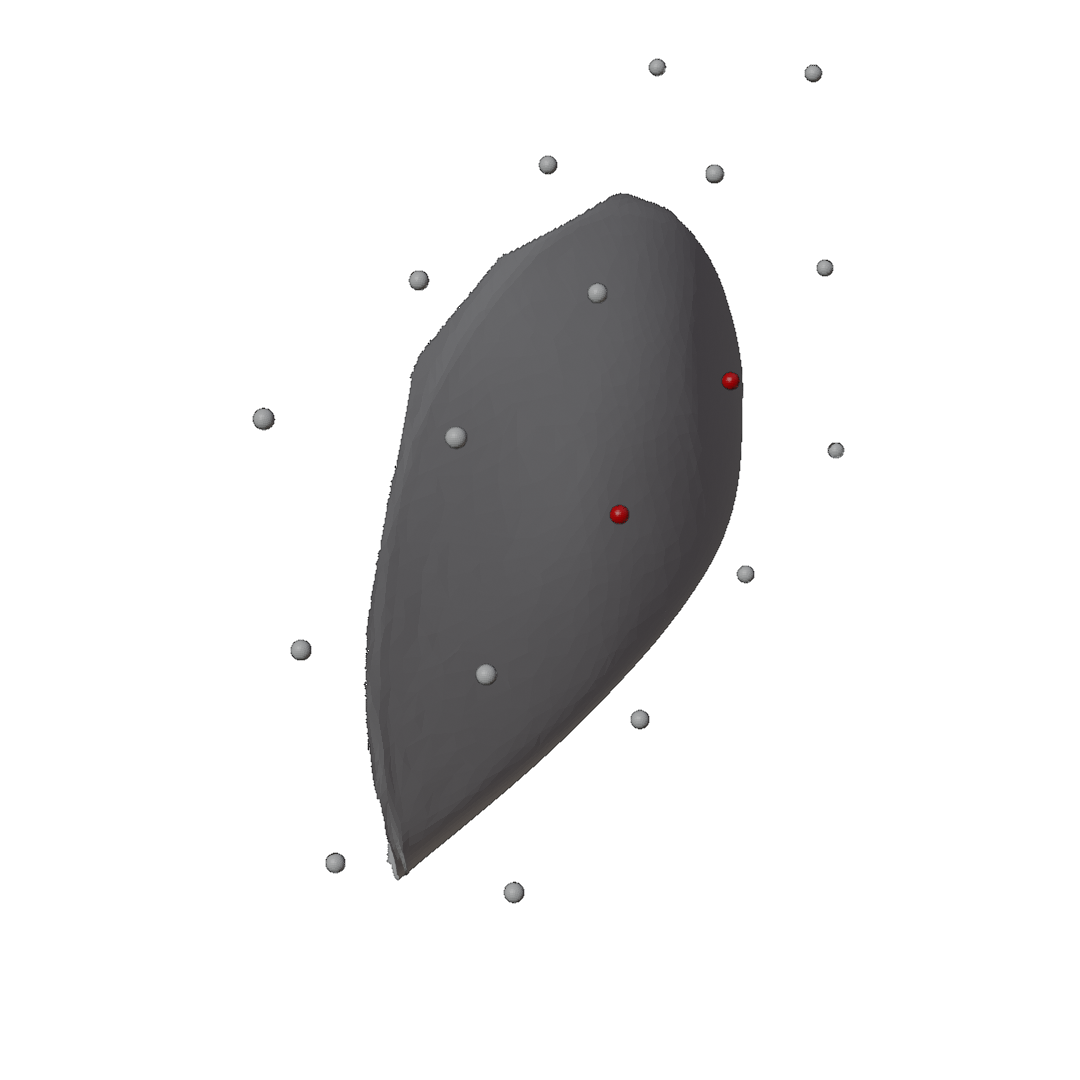
\includegraphics[width=.7\linewidth]{bilder/2ptDeformationPoints}
	\caption{Deformationspunkte des ersten Experiments}
	\label{fig:ffd1st}
\end{figure}
Auch wurde die Laufzeit soweit beschränkt, dass sinnvolle Aussagen darüber getroffen werden können, ob und wie gut der Algorithmus lernt, für finale Ergebnisse hingegen wäre die Anzahl an Samples die ausgewertet werden sowie die Anzahl an Genrationen für Akquise, und finaler Auswertung höher zu wählen.
Um bewerten zu können ob die Einbindung des Constraints einen Effekt auf den Algorithmus hat, und um diesen Effekt quantifizieren zu können wurde der Algorithmus unter den in Tabelle \cref{tab:param1st} beschriebenen Parametern sowohl mit Constraint als auch ohne Constraint durchgeführt. 
\begin{figure}[h]
	\centering
	\begin{minipage}{0.45\textwidth}
		\centering
		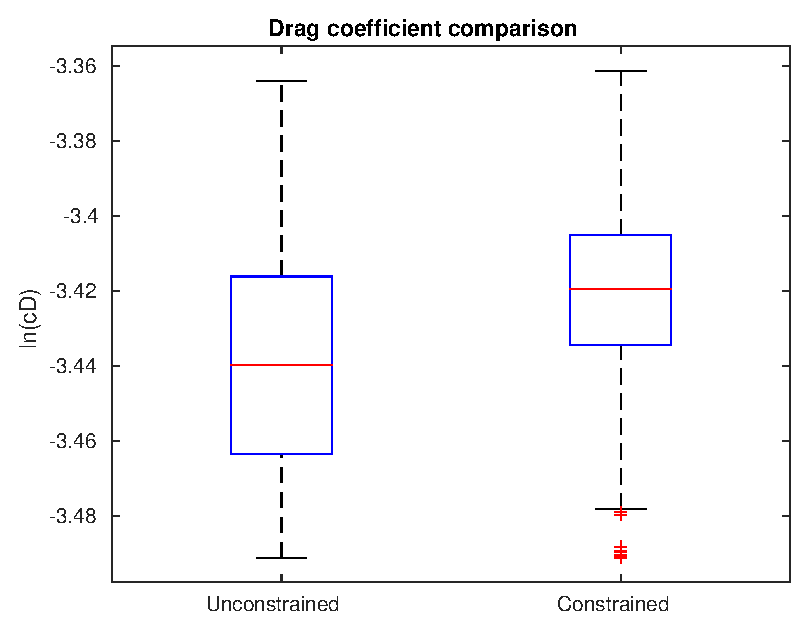
\includegraphics[width=1\linewidth]{bilder/2pt500Samples/dragBoxplot}
		\caption{Comparison of final drag values}
		\label{fig:1stdragbox}
	\end{minipage}\hfill
	\begin{minipage}{0.45\textwidth}
		\centering
		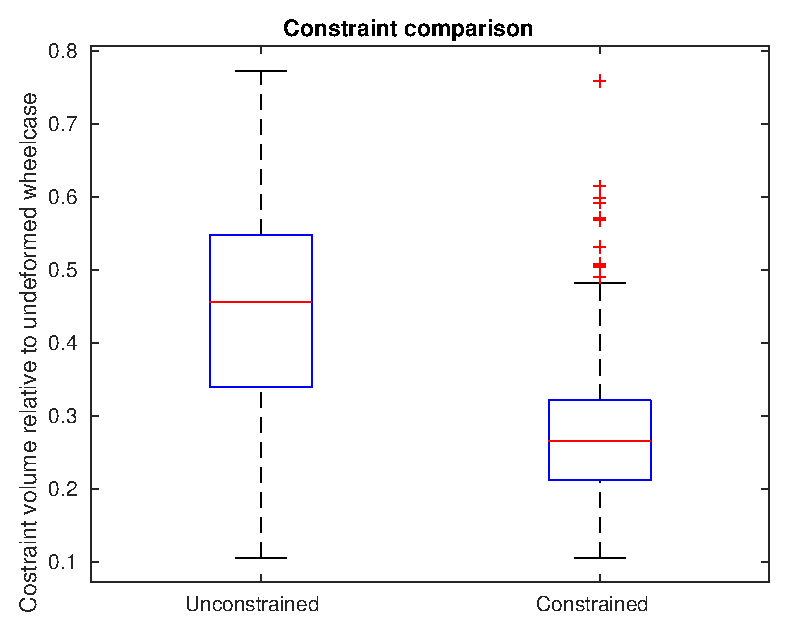
\includegraphics[width=1\linewidth]{bilder/2pt500Samples/constraintBoxplot}
		\caption{Comparison of final constraint values}
		\label{fig:1stconbox}
	\end{minipage}
\end{figure}

Die Ergebnisse des ersten Experiments sehen vielversprechend aus In Abb. \cref{fig:1stdragbox} ist ein Vergleich der Luftwiderstandsergebnisse 
\footnote{Im Experiment wurde statt der direkten Luftwiderstandswerte, der natürliche Logarithmus dieser genutzt.} 
der erzeugten Lösungen abgebildet.
Die erste Beobachtung die gemacht werden kann, ist dass die produzierten Werte aus der Variante mit Constraint in der gleichen Größenordnung liegen wie die aus der Variante ohne Constraint.
Der Algorithmus scheint also auch mit Constraint noch korrekt zu lernen.
Es ist zu Erkennen, dass die Einbindung des Constraints zu einer Verschlechterung der Luftwiderstandswerte führt, eine Verschlechterung dieser durch eine Fokussierung auf zwei Ziele ist allerdings zu erwarten.
Trotzdem muss betont werden, dass die Verschlechterung erstaunlich klein ist, so beträgt der relative Unterschied zwischen dem Median der Version mit Constraint und dem Median der Version ohne nur \todo{genaue zahl}.

Um eine solche Verschlechterung zu rechtfertigen sollte die Qualität des Sekundärziels herangezogen werden.
Dazu ist in \cref{fig:1stconbox} ein Vergleich bezüglich des Constraintvolumens dargestellt.
Die erste Beobachtung hier ist, dass die Einbindung des Constraints zu einer stärkeren Beachtung dessen führt.
Das ist offensichtlich das Ziel bei der Nutzung eines Constraints, dass diese Erwartung erfüllt wird zeigt, dass die Formulierung des Constraints insofern korrekt ist, dass eine Verbesserung dieses erreicht werden kann.
Auch ist hervorzuheben, dass die relative Verbesserung des Constraints wesentlich stärker ist als die relative Verschlechterung des Luftwiderstands.
Eine Verschlechterung des Medians bezüglich des Luftwiderstands von \todo{genaue zahl} geht hier mit einer Verbesserung des Medians bezüglich des Constraints von \todo{genaue zahl} einher.

Interessant sind auch die Grenzen der Verteilungen, beide Verteilungen weisen eine untere Grenze von ca. 0.1, sprich 10\% des Außenvolumens des unverformten Radkastens auf.
Dies lässt sich dadurch erklären, dass das Radausschlagsvolumen einen Teil unterhalb des Radkastens hat, der durch eine seitliche Deformation des Radkastens nicht eliminiert werden kann.
Die zweite interessante Grenze stellt die Obergrenze von 0.8 dar.
Selbst die schlechteste Lösung in der Version ohne Constraint ist damit besser als der undeformierte Radkasten.
Dies kann einerseits an zu eng gewählten Deformationsparametern liegen, die genutzte Konfiguration erlaubte allerdings Deformationen nach innen.
Die plausiblere Hypothese ist, dass die Wahl der Breite des Radkastens als Feature bedeutet, dass eine Minimalbreite existiert, bei der nicht das Zentrum des Radkastens, sondern die Ränder den breitesten Punkt darstellen.
Jede Deformation die das Zentrum stärker nach innen verformt, würde in die gleiche Zelle der Karte eingeordnet werden.
Wenn weniger stark verformte Radkästen bezüglich deren Fitness optimaler sind, wird dies dazu führen, dass Radkästen mit einer stärkeren Verformung nach innen keinen Einzug in die Karte finden können.

Aufgrund der Tatsache, dass SAIL ein divergenter Optimierungsalgorihtmus ist haben die finalen Verteilungen nur eingeschränkte Aussagekraft.
Besonders dadurch, dass das Feature der Breite des Velomobils mit der Schwierigkeit der Erfüllung des Constraints korreliert ist, müssen auch die produzierten Karten analysiert werden.

\begin{figure}[h]
	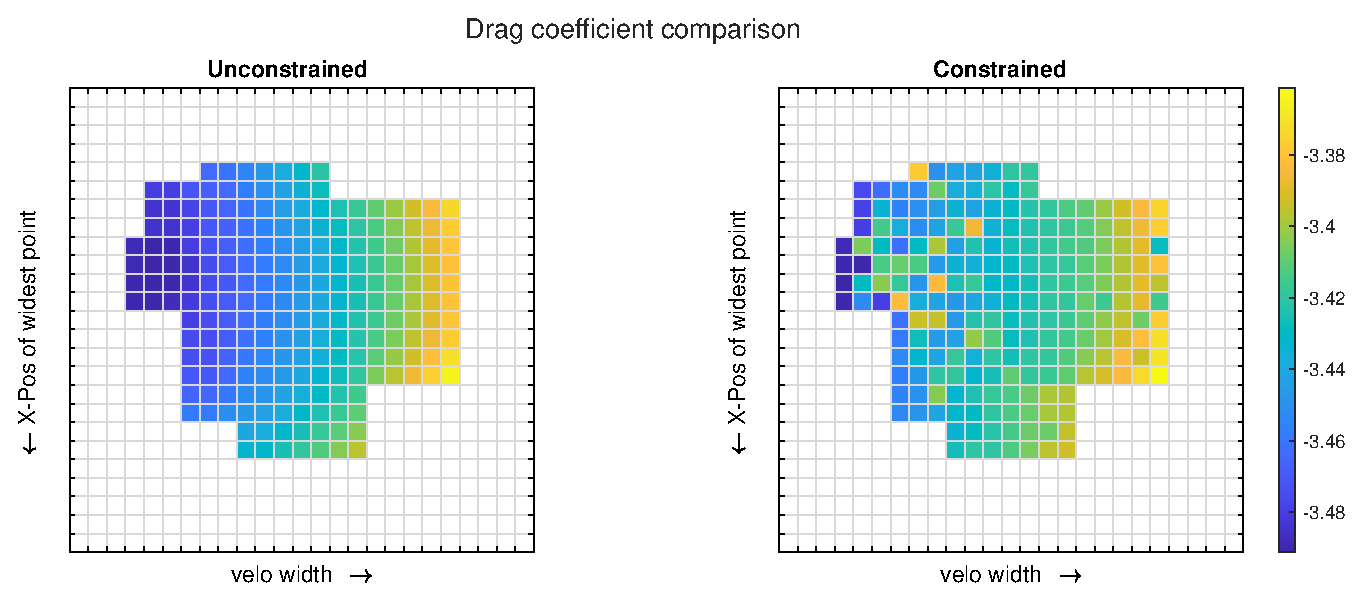
\includegraphics[width=1\linewidth]{bilder/2pt500Samples/dragMapComparison}
	\caption{Maps of final drag values}
	\label{fig:1stmapDrag}
\end{figure}

In Abb. \cref{fig:1stmapDrag} sind die Karten von Luftwiderstandskoeffizienten der produzierten Ergebnisse in beiden Versionen aufgeführt.
Die Karte ohne Constraint bestätigt die Hypothese, dass breitere Velomobile mit schlechterem Luftwiderstandskoeffizienten korreliert sind.
Auch ist erkennbar, dass es ein mittleres Optimum bezüglich der x-Position dieses Punktes zu geben scheint, da Luftwiderstandswerte sowohl bei Abweichungen nach oben als auch bei Abweichungen nach unten schlechter werden.
Dass die oben aufgestellte Hypothese bestätigt werden kann und die Karte einen graduellen Verlauf aufweist, sind Zeichen für die korrekte Funktionalität des Algorithmus.
Im Gegensatz dazu ist die Karte der Variante mit Constraint wesentlich unregelmäßiger.
Dies bedeutet allerdings nicht, dass der Algorithmus in dieser Variante nicht korrekt arbeitet, die Unregelmäßigkeit der Karte rührt daher, dass die Fitness des Algorithmus aus einer Kombination von Luftwiderstandskoeffizienten und Constraint zusammensetzt.
Auch bewegen sich die Luftwiderstandswerte, wie bereits anhand der Boxplots sichtbar war im Bereich.
Besonders gute Lösungen bezüglich einer dieser beiden Komponenten können fehlende Optimalität bezüglich der anderen damit ausgleichen.
Trotzdem sind auch in dieser Karte die gleichen zugrundeliegenden Tendenzen zu erkennen, breitere Velomobile sind auch hier schlechter bezüglich des Luftwiderstands sind und Optimalität sinkt nach unten und oben.
Interessant ist, dass am rechten, sprich breiteren, Ende einige Lösungen gefunden wurden die sogar bessere Luftwiderstandswerte aufweisen als deren Gegenstücke in der Variante ohne Constraint.
Und auch wenn auf der linken Seite einige Lösungen existieren, welche erheblich schlechtere Luftwiderstandswerte aufweisen wie ihre Gegenstücke, so existieren auch sehr viele mit vergleichbaren Werten.
Um solche Verschlechterungen in Kontext setzten zu können müssen sich die Karten des Constraints angeschaut werden.

\begin{figure}[h]
	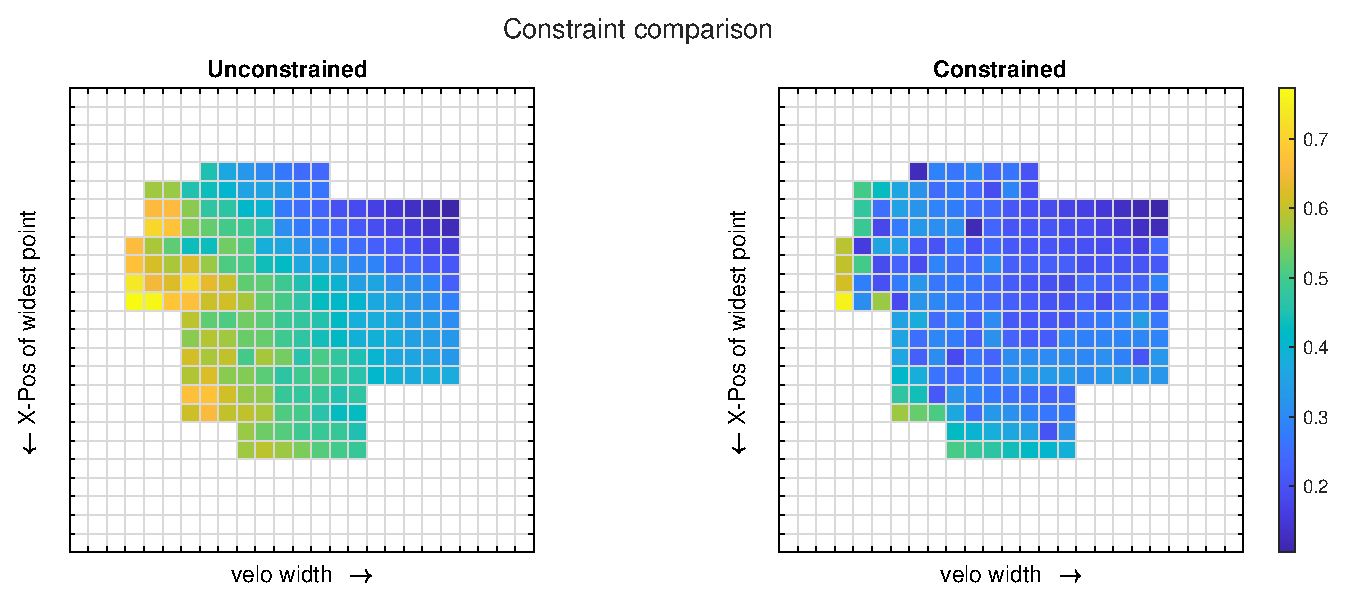
\includegraphics[width=1\linewidth]{bilder/2pt500Samples/constraintMapComparison}
	\caption{Maps of final constraint values}
	\label{fig:1stmapCon}
\end{figure}

In Abb. \cref{fig:1stmapDrag} sind die Karten der korrespondierenden Constraint-Werte für beide Varianten zu sehen.
Ersteinmal lässt sich auch hier die Hypothese bestätigen, dass breitere Velomobile den Constraint besser erfüllen.
Interessant ist allerdings auch, dass ohne Einbindung des Constraints, Lösungen, deren breitester Punkt weiter vorne ist den Constraint besser erfüllen.

Im Vergleich der beiden Karten ist noch viel stärker, als den Boxplots, ersichtlich welchen Effekt die Einbindung des Constraints hat.
Es ist klar ersichtlich wie viel besser ein Großteil der Lösungen den Constraint erfüllen.
Besonders stark is dieser Effekt im Mittelfeld der Karte in denen sich Constraintwerte halbieren und teilweise noch stärker verringern.
Zum rechten extremen Rand schwächt die Constraintverbesserung ab, da dortige Radkästen so breit sind, dass selbst die Variante ohne Constraint diesen leicht erfüllen kann.
Auch ist hervorzuheben, dass sich Verbesserungen bis zum linken Rand der Individuen durchziehen.
Selbst in der linken, sprich schmalsten Spalte, ist eine Verbesserung der Individuen erkennbar, und die nächste Spalte enthält bereits ein Individuum welches nahe der besten gefundenen Constraint-Werte angesiedelt ist.

\begin{figure}[h]
	\centering
	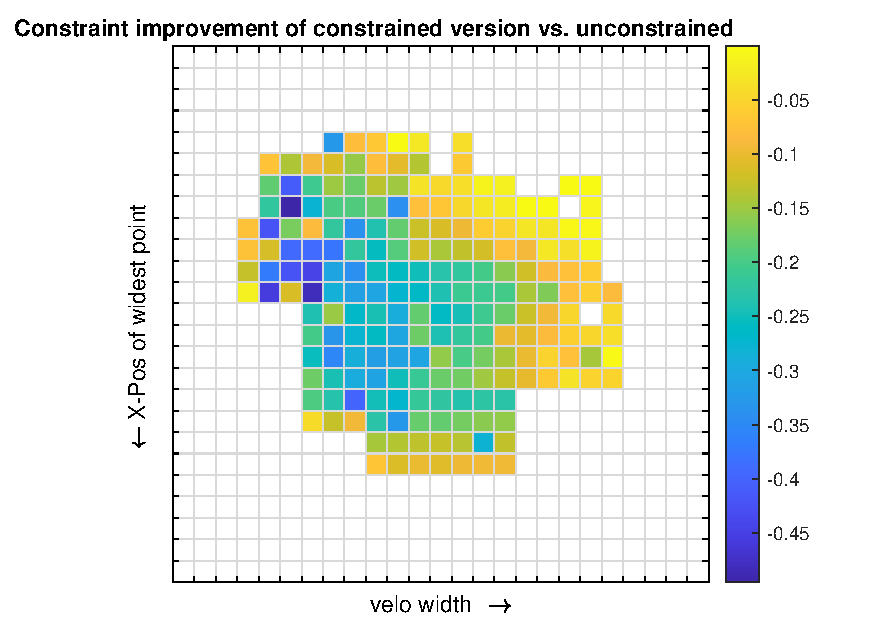
\includegraphics[width=.7\linewidth]{bilder/2pt500Samples/constraintImprovements}
	\caption{Maps of final constraint values}
	\label{fig:1stmapConCompare}
\end{figure}

In Abb. \cref{fig:1stmapConCompare} ist die Verbesserung der Constraintwerte von der Version ohne Constraint zur Version mit Constraint dargestellt.
Der bereits oben erwähnte Effekt, dass die größten Verbesserungen besonders in der linken Hälfte der Karte stattfinden ist hier noch klarer ersichtlich.
Gerade diese Hälfte ist allerdings die, die bessere Luftwiderstandswerte aufweist und in der die Erfüllung des Constraints aufgrund der geringeren Breite, die Velomobile in diesen Zellen auszeichnet, wesentlich schwerer fällt.
%\begin{figure}[h]
%	\centering
%	\begin{minipage}{0.45\textwidth}
%		\centering
%		\includegraphics[width=1\linewidth]{bilder/2pt500Samples/bestUn}
%		\caption{Comparison of final drag values}
%		\label{fig:1stdragbox}
%	\end{minipage}\hfill
%	\begin{minipage}{0.45\textwidth}
%		\centering
%		\includegraphics[width=1\linewidth]{bilder/2pt500Samples/best}
%		\caption{Comparison of final constraint values}
%		\label{fig:1stconbox}
%	\end{minipage}
%\end{figure}
Zusammenfassend kann man sagen, dass die Einbindung des Constraints mit den im ersten Experiment vorliegenden Einschränkungen merkliche Auswirkungen auf das Ergebnis hat.
Auch ist herauszustellen, dass eine starke Verbesserung des Constraints bei einer schwachen Verschlechterung des Luftwiderstands stattfindet.
%Weiterführenden Experimente sollten ohne die Einschränkungen bezüglich Freiheitsgraden und Länge des Experimentes

\subsubsection{Erhöhung der Freiheitsgrade}

Mit dem ersten Experiment konnte gezeigt werden, dass der Algorithmus sowohl Luftwiderstandskoeffizienten als auch Constraint optimiert, und dabei relativ geringe Kosten in Bezug zum erreichten Luftwiderstand entstehen.
Das erste Experiment hatte allerdings einige Einschränkungen, bezüglich der Parametrisierung um es einfach zu halten.
Die erste dieser Einschränkungen war die Reduzierung auf Deformation in 2 Punkten, sprich 6 Freiheitsgraden.
Diese Reduzierung half dabei das Problem klein zu halten, hatte aber eine erhebliche Einschränkung des Lösungsraums zur Folge.
Ziel des zweiten Experiments ist es die Anzahl an Freiheitsgraden erheblich zu erhöhen, damit die Zahl an möglichen Deformationen erheblich zu erhöhen, was den positiven Effekt der Einbindung eines Constraints hoffentlich verstärkt.

\begin{figure}[h]
	\centering
	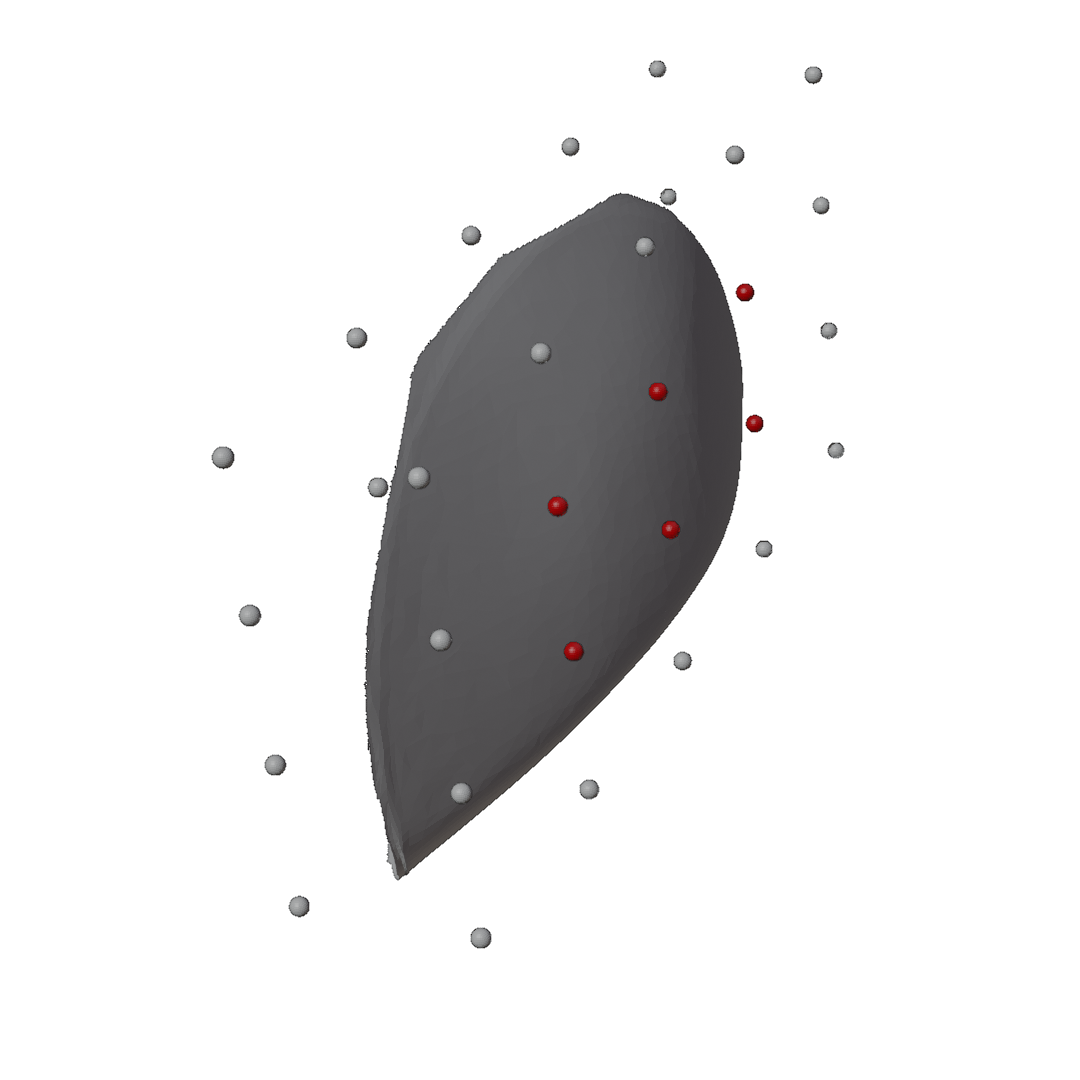
\includegraphics[width=.7\linewidth]{bilder/6ptDeformationPoints}
	\caption{Deformationspunkte des 2. Experiments}
	\label{fig:ffd2nd}
\end{figure}
Die in \todo{} dargestellte Freiheitsgrade wurden mit einigen Vorüberlegungen gewählt.
Die Anzahl an horizontaler Reihen wurde von einer auf zwei erhöht um Deformationen , wie eine Auseinanderziehen oder Zusammendrücken in z-Richtung zu erlauben.
Es liegt die Vermutung nahe, dass die im vorigen Experiment gewählten Deformationspunkte die möglichen Phänotypen einschränken, besonders in Anbetracht auf die x-Position des breitesten Punkts.
Da diese eine der Features der MAP-Elites-Karte ist, und die Karte im vorigen Experiment entlang dieser Dimension nicht vollständig ausgefüllt wurde, wurde die Anzahl der Deformationspunkte in x-Richtung von 2 auf drei erhöht, um mehr Deformationen zuzulassen, in denen der breiteste Punkt weiter vorne oder hinten liegt.
Insgesamt ergeben sich dadurch 6 Deformationspunkte, welche in alle drei Richtungen bewegt werden können, wodurch sich 18 Freiheitsgrade ergeben.
%Diese Erhöhung ist groß genug

\begin{table}[h]
	\centering
	\begin{tabularx}{.75\textwidth}{ll}\hline
		Anzahl initialer Samples & 100 \\
		Anzahl Samples & 500 \\
		Anzahl neuer Samples pro Akquiseschleife & 20 \\
		Anzahl Generationen Akquise-MAP-Elites & 1024 \\
		Kinder pro Generation Akquise-MAP-Elites & 32 \\
		Anzahl Generationen Ergebnis-MAP-Elites & 2048 \\
		Kinder pro Generation Akquise-MAP-Elites & 32 \\
		Auflösung der MAP-Elites Karte & 25 * 25  \\
		\hline
		%\rowcolor{lightgray}
		Freiheitsgrade & 18 \\
		Mittelwertgewichtung & 1 \\
		Varianzgewichtung & 2 \\
		Constraintgewichtung & 1 \\
	\end{tabularx}
	\label{tab:param2nd}
	\caption{Parametrisierung des zweiten Experiments (Änderungen zum ersten Experiment hervorgehoben)}
\end{table}


\begin{figure}[h]
	\centering
	\begin{minipage}{0.45\textwidth}
		\centering
		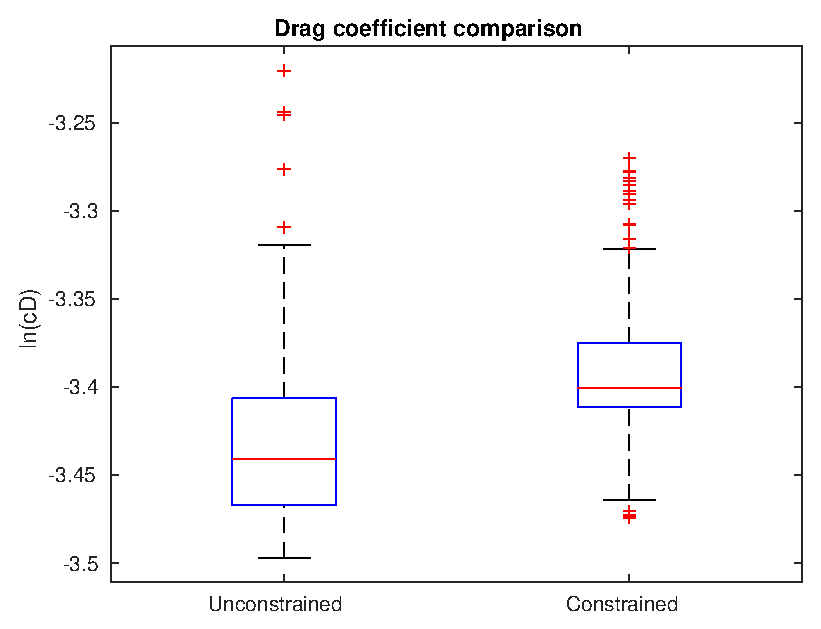
\includegraphics[width=1\linewidth]{bilder/6pt500Samples/dragBoxplot}
		\caption{Comparison of final drag values}
		\label{fig:2nddragbox}
	\end{minipage}\hfill
	\begin{minipage}{0.45\textwidth}
		\centering
		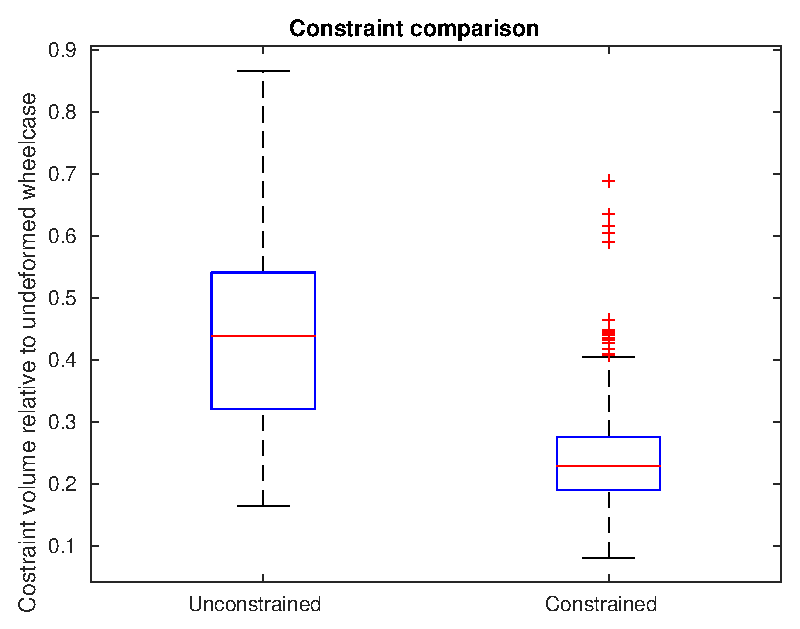
\includegraphics[width=1\linewidth]{bilder/6pt500Samples/constraintBoxplot}
		\caption{Comparison of final constraint values}
		\label{fig:2ndconbox}
	\end{minipage}
\end{figure}

Der erste Unterschied, der im Vergleich zum ersten Experiment auftritt, sind die stärkeren Unterschiede in Constraint und Luftwiderstand für.


\begin{figure}[h]
	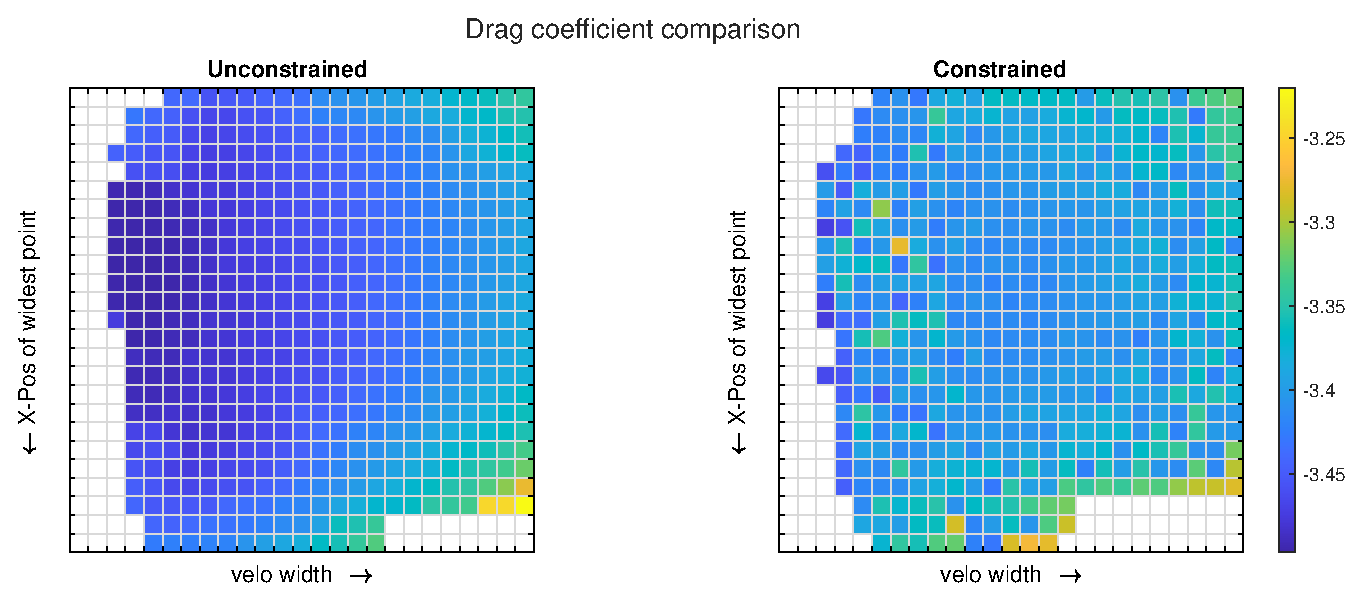
\includegraphics[width=1\linewidth]{bilder/6pt500Samples/dragMapComparison}
	\caption{Maps of final drag values}
	\label{fig:2ndmapDrag}
\end{figure}

In Abbildungen \cref{fig:2ndmapCon} \cref{fig:2ndmapDrag} ist klar zu Erkennen, dass die Karte aus Lösungen weitaus besser gefüllt wird als beim ersten Experiment.
Die bessere Füllung entlang der Vertikalen ist leicht zu erklären.
Die Aufteilung in 6 Deformationspunkte führt dazu, dass die beiden vorderen weiter vorne liegen, als der vordere aus dem vorigen Experiment und die beiden hinteren entsprechend auch weiter hinten liegen.
Deformationen mit diesen Deformationspunkten können also mehr Lösungen generieren, in denen der breiteste Punkt sehr weit vorne oder sehr weit hinten liegt.
Interessant ist allerdings, dass die Karte auch entlang der Horizontalen  besser gefüllt wird.
An der Stärke der Deformationen in y-Richtung wurde allerdings nichts geändert, es sollte also nicht möglich sein wesentlich breitere Velomobile zu generieren.
\todo{Erklärung warum mehr horiz}

\begin{figure}[h]
	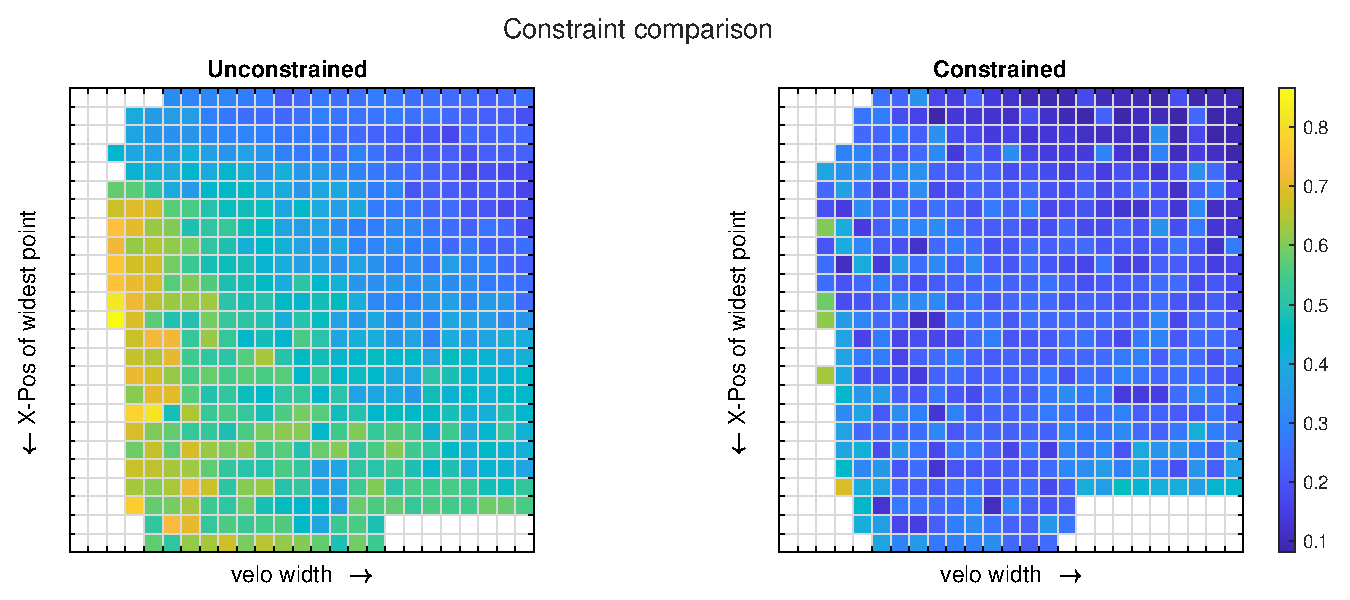
\includegraphics[width=1\linewidth]{bilder/6pt500Samples/constraintMapComparison}
	\caption{Maps of final constraint values}
	\label{fig:2ndmapCon}
\end{figure}

Die Karte der Constraints bestätigt auch hier, die im ersten Experiment bereits beobachtete Tendenz, dass der Constraint in breiteren Velomobilen und in solchen in denen der breiteste Punkt weiter vorne liegt einfacher zu erfüllen ist.
Es ist allerdings herauszustellen, dass in der Variante ohne Constraint selbst die Lösungen in der oberen rechten Ecke eine weniger gute Constrainterfüllung aufweisen als die besten Lösungen in der Variante ohne Constraint des ersten Experiments, trotz der Tatsache, dass diese sowohl breiter sind und die breiteste Stelle weiter vorne liegt.
Zwar ist dieser Effekt auch im Vergleich der Varianten ohne Constraint festzustellen, er fällt dort aber wesentlich schwächer aus.
Dies deckt sich mit der Tatsache, dass eine Erhöhung der Freiheitsgrade und die damit verbundene Vergrößerung des Suchraumses schwerer macht ähnlich gute Lösungen bei gleicher Laufzeit zu finden.
Dass der Effekt in der Variante ohne Constraint aber stärker ist bestätigt, dass die Schwierigkeit des zufälligen Erfüllen des Constraints ohne spezielle Behandlung stärker wächst, als die Schwierigkeit der Erfüllung unter Beachtung des Constraints.

\begin{figure}[h]
	\centering
	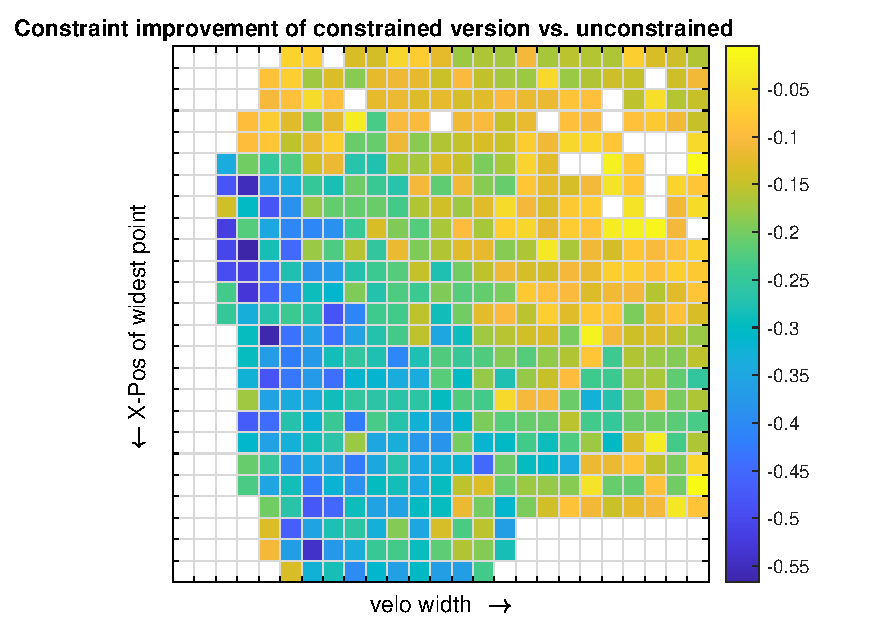
\includegraphics[width=.7\linewidth]{bilder/6pt500Samples/constraintImprovements}
	\caption{Maps of final constraint values}
	\label{fig:2ndmapConCompare}
\end{figure}

Es fällt eine interessanter Unterschied zum ersten Experiment auf.
Die Karten der Variante ohne Constraint und der mit Constraint sind im Gegensatz diesen nicht mehr gleich.
Stattdessen ist die Karte ohne Constraint besser gefüllt als die mit Constraint.
Dies fällt vor allem an den Rändern der Karten auf.
Das kann damit zusammenhängen, dass durch die Einführung des Constraints Exploration in Bereichen in denen der Constraint verletzt ist weniger stattfindet.
Außerdem besteht die Vermutung, dass weite Teile des Problemraums den Constraint nicht erfüllen, sondern stark verletzen.

\missingfigure{boxplots akquiseindividuen}

Zur definitiven Auswertung sollte allerdings sichergestellt sein, dass Akquise- und Ergebnis-MAP-Elites ausreichend auskonvergiert sind.
Dass kann aus in diesem Experiment noch nicht definitiv festgestellt werden.
Um eine definitive Aussage über Konvergenz treffen zu können sollte das Experiment unter ausführlicheren Bedingungen wiederholt werden.

\subsubsection{Erhöhung der Laufzeit}

Das zweite Einschränkung der beiden vorigen Experimente war die Beschränkung auf eine kleinere Anzahl an ausgewerteten Samples und Generationen in Akquise- und Ergebnis-MAP-Elites.
Durch die Beschränkung auf eine kleinere Anzahl an Samples besteht die Möglichkeit, dass der Suchraum nicht präzise genug und/oder nicht weitläufig genug abgebildet wurde.
Die Beschränkung in Generationen des Akquise- und Ergebnis-MAP-Elites kann dazu führen, dass diese noch nicht vollständig auskonvergiert sind.
Da die Überlegung nahe liegt, dass die Variante mit Constraint länger benötigen könnte um auszukonvergieren, sollte untersucht werden ob die Erhöhung dieser Parameter zu signifikanten Änderung im Vergleich zur kürzeren Version führt, indem die Gewinne nach 500 Samples und 1024 bzw. 2048 Generationen quantifiziert werden.

\begin{table}[h]
	\centering
	\begin{tabularx}{.75\textwidth}{ll}\hline
		Anzahl initialer Samples & 100 \\
		%\rowcolor{lightgray}
		Anzahl Samples & 1000 \\
		Anzahl neuer Samples pro Akquiseschleife & 20 \\
		%\rowcolor{lightgray}
		Anzahl Generationen Akquise-MAP-Elites & 2048 \\
		Kinder pro Generation Akquise-MAP-Elites & 32 \\
		%\rowcolor{lightgray}
		Anzahl Generationen Ergebnis-MAP-Elites & 8192 \\
		Kinder pro Generation Akquise-MAP-Elites & 32 \\
		Auflösung der MAP-Elites Karte & 25 * 25  \\
		\hline
		Freiheitsgrade & 18 \\
		Mittelwertgewichtung & 1 \\
		Varianzgewichtung & 2 \\
		Constraintgewichtung & 1 \\
	\end{tabularx}
	\label{tab:params3rd}
	\caption{Parametrisierung des dritten Experiments (Änderungen zum zweiten Experiment hervorgehoben)}
\end{table}

Auf ersten Blick sehen die Ergebnisse des dritten Experiments denen des zweiten Experiments sehr ähnlich.
Die Karten werden etwas besser gefüllt, was durch Erhöhung der Zahl der ausgewerteten Samples und der Akquise- und Ergebnisgenerationen grundsätzlich zu erwarten war.

\begin{figure}[h]
	\centering
	\begin{minipage}{0.45\textwidth}
		\centering
		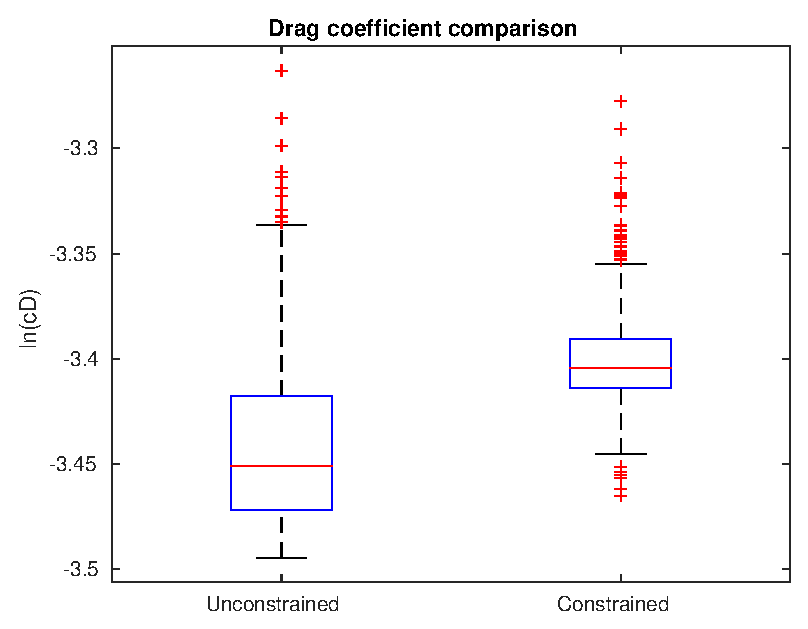
\includegraphics[width=1\linewidth]{bilder/6pt1000Samples/dragBoxplot}
		\caption{Comparison of final drag values}
		\label{fig:3rddragbox}
	\end{minipage}\hfill
	\begin{minipage}{0.45\textwidth}
		\centering
		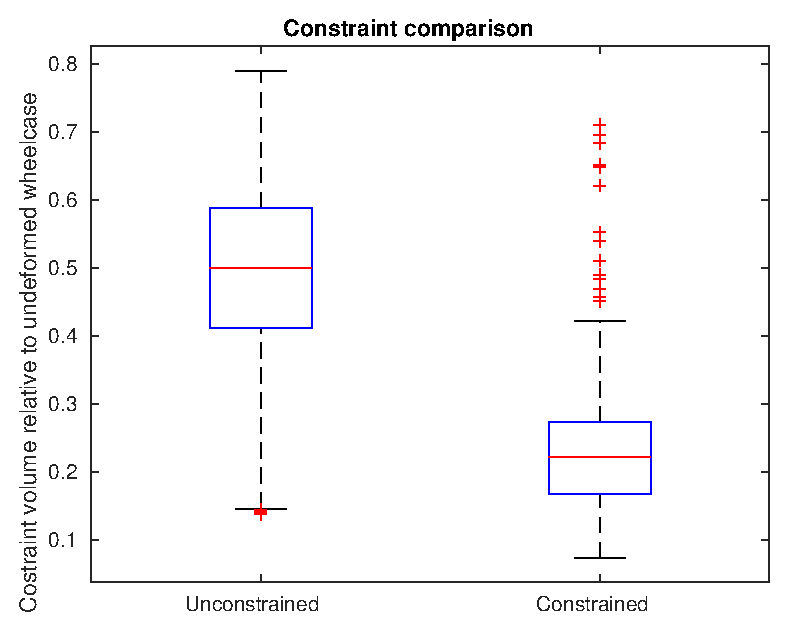
\includegraphics[width=1\linewidth]{bilder/6pt1000Samples/constraintBoxplot}
		\caption{Comparison of final constraint values}
		\label{fig:3rdconbox}
	\end{minipage}
\end{figure}

Die Luftwiderstandskoeffizienten der Variante ohne Constraint haben sich nicht verändert, während bei der Variante mit Constraint ist eine leichte Verbesserung zu verzeichnen.
Dies deckt sich mit der Vermutung, dass die Variante mit Constraint mehr Zeit benötigt um ausreichend auszukonvergieren.
Interessant ist auch die Veränderung der Constraintwerte.
Hier ist bei der Variante mit Constraint keine redenswerte Änderung zu verzeichnen, die Constraintwerte der Variante ohne Constraint verschlechtern sich allerdings.
Das ist durchaus interessant, da es bedeuten kann dass die weitere feine Optimierung bezüglich des Luftwiderstands im Laufe des Algorithmus eine Abkehr von solchen Lösungen darstellt, die den Constraint besser erfüllen.
Das dieser Trend in der Variante ohne Constraint nicht zu beobachten ist ein großer Vorteil.
Auch ist das interessant, da kein nenneswerter Gewinn bezüglich des Luftwiderstands zischen ersten und zweitem Experiment zu beobachten ist.

\begin{figure}[h]
	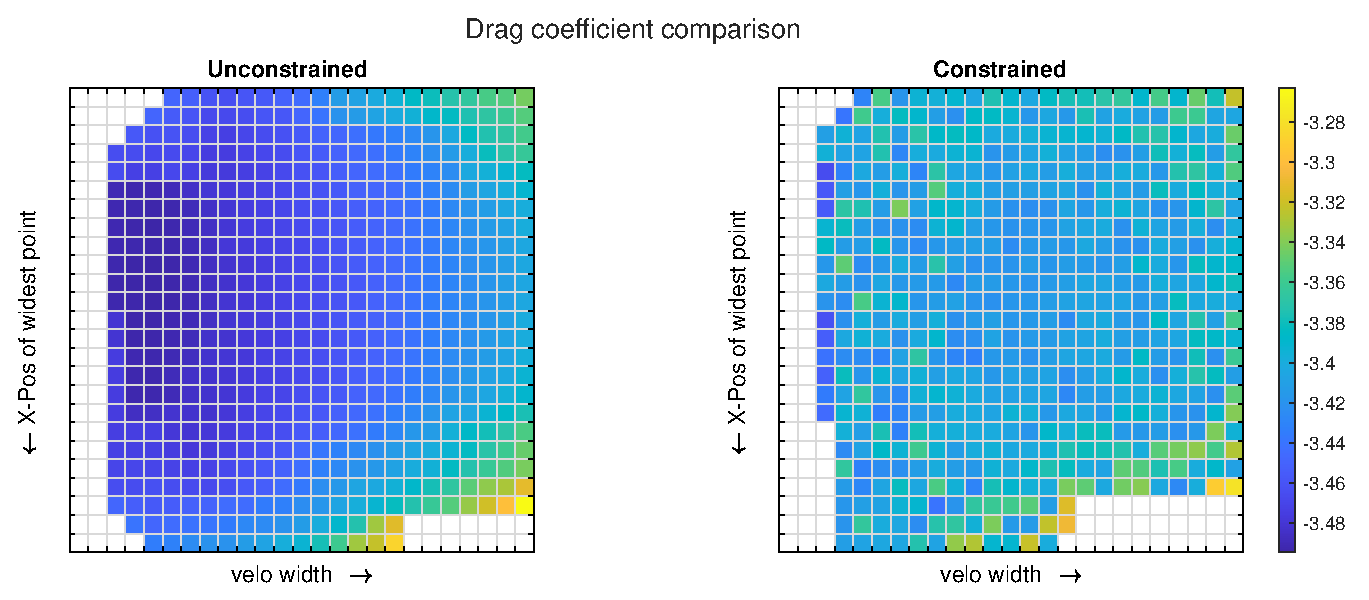
\includegraphics[width=1\linewidth]{bilder/6pt1000Samples/dragMapComparison}
	\caption{Maps of final drag values}
	\label{fig:3rdmapDrag}
\end{figure}


\begin{figure}[h]
	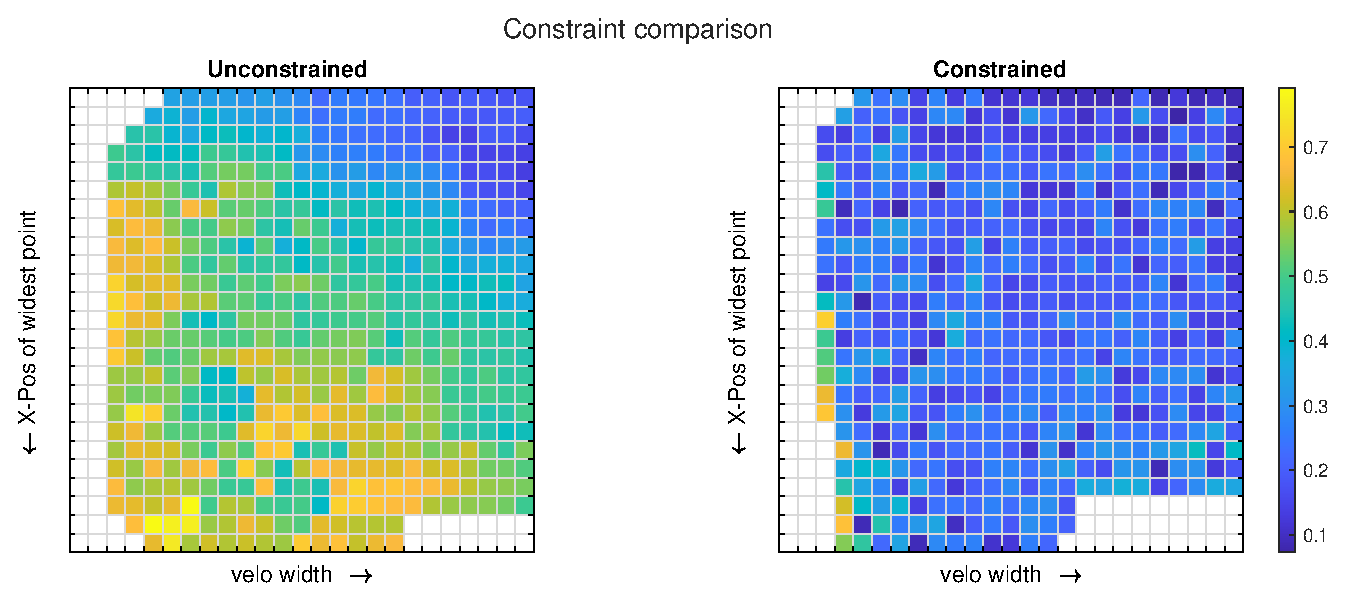
\includegraphics[width=1\linewidth]{bilder/6pt1000Samples/constraintMapComparison}
	\caption{Maps of final constraint values}
	\label{fig:3rdmapCon}
\end{figure}


\subsubsection{Zusammenfassung}


%\subsection{E-Roller}
%\subsubsection{Experimente}
%\subsubsection{Analyse}
%\subsubsection{Zusammenfassung}


%\begin{figure}
%	\begin{tabularx}{.75\textwidth}{ll}\hline
%		Anzahl initialer Samples &  \\
%		Anzahl Samples &  \\
%		Anzahl neuer Samples pro Akquiseschleife & \\
%		Anzahl Generationen Akquise-MAP-Elites & \\
%		Kinder pro Generation Akquise-MAP-Elites & \\
%		Anzahl Generationen Ergebnis-MAP-Elites & \\
%		Kinder pro Generation Akquise-MAP-Elites &  \\
%		Auflösung der MAP-Elites Karte &   \\
%		\hline
%		Freiheitsgrade &  \\
%		Mittelwertgewichtung & 1 \\
%		Varianzgewichtung & 2 \\
%		Constraintgewichtung & 1 \\
%	\end{tabularx}
%\end{figure}
